\documentclass[12pt]{article}

\usepackage{sbc-template}
\usepackage{graphicx,url}
\usepackage[utf8]{inputenc}
%\usepackage[brazil]{babel}
\usepackage[english]{babel}

\usepackage{amsmath,amssymb}

\usepackage[caption=false]{subfig}
\usepackage{braket}
\usepackage{amsfonts}
\usepackage{amsthm}
\usepackage{fancyhdr}
\usepackage{comment}
\usepackage{float}
\usepackage{mathtools}
\usepackage{xspace}

%\usepackage[latin1]{inputenc}  

\newtheorem{theorem}{Theorem}
\newtheorem{lemma}[theorem]{Lemma}
\newtheorem{definition}[theorem]{Definition}
\newtheorem{corollary}[theorem]{Corollary}
\newtheorem{cor}[theorem]{Corollary}
\newtheorem{prop}[theorem]{Proposition}
\newtheorem{fact}[theorem]{Fact}
\renewcommand{\proofname}{Proof}

     
\sloppy

\title{On the Helly Property of  Some Intersection Graphs}

\author{Tanilson D. Santos\inst{1,2},\\ Orientador: Jayme L. Szwarcfiter\inst{1,3,4},\\ Co-orientadores: Claudson F. Bornstein\inst{1,3}, Uéverton S. Souza\inst{5} }


\address{Computer and Systems Engineering Program\\ Federal University of Rio de Janeiro (PESC/Coppe/UFRJ) 
%Avenida Horácio Macedo 2030, Centro de Tecnologia, Bloco H, sala 319\\
%Cidade Universitária - CEP: 21941-914 
\nextinstitute
  Course of Computer Science\\ Federal University of Tocantins (UFT)
\nextinstitute
Departament of Computer Science\\
Mathematics Institute\\
Federal University of Rio de Janeiro (IM/UFRJ)
\nextinstitute
Departament of Mathematics\\
State University of Rio de Janeiro (UERJ)
\nextinstitute
Computing Institute\\
Fluminense Federal University (UFF) 
  \email{tanilson.dias@uft.edu.br,
  \{jayme@nce, cfb@dcc\}.ufrj.br,
  ueverton@ic.uff.br}
}

\begin{document} 

\maketitle

\begin{abstract}
  An EPG graph  $G$  is an edge-intersection graph of paths on a grid. 
In this summary of doctoral thesis we mainly explore the  EPG graphs, in particular $B_1$-EPG graphs. However, other classes of intersection graphs were studied such as VPG, EPT and VPT graph classes, in addition to the parameters Helly number and strong Helly number to EPG and VPG graphs. We  present a proof of $NP$-completeness to Helly-$B_1$-EPG graph recognition problem. We completely solve the problem of determining the Helly and strong Helly numbers, in both graph classes $B_k$-EPG, and $B_k$-VPG graphs, for each value $k$. Last but not least,  we present the result that every Chordal $B_1$-EPG graph is simultaneously in the VPT and EPT graph classes. 
\end{abstract}
     
% \begin{resumo} 
%   Este meta-artigo descreve o estilo a ser usado na confecção de artigos e
%   resumos de artigos para publicação nos anais das conferências organizadas
%   pela SBC. É solicitada a escrita de resumo e abstract apenas para os artigos
%   escritos em português. Artigos em inglês deverão apresentar apenas abstract.
%   Nos dois casos, o autor deve tomar cuidado para que o resumo (e o abstract)
%   não ultrapassem 10 linhas cada, sendo que ambos devem estar na primeira
%   página do artigo.
% \end{resumo}


\section{Introduction}

Models based on paths intersection  may consider  intersections by vertices or   intersections by edges.  Cases where the paths are hosted on a tree  appear first in the literature, see for instance \cite{gavril1978recognition, golumbic1985}.  Representations using paths on a grid were considered later, see  \cite{golumbic2009,golumbic2013}.

 Let $P$ be a family of paths on a host tree $T$. Two types of intersection graphs from the pair $<P,T>$ are defined, namely VPT and EPT graphs.
The \textit{edge intersection graph} of $P$, EPT(P), has vertices which correspond to the members of $P$, and two vertices are adjacent in EPT(P) if and only if the corresponding paths in $P$ share at least one edge in T. Similarly, the \textit{vertex intersection graph} of $P$, VPT(P), has vertices which correspond to the members of $P$, and two vertices are adjacent in VPT(P) if and only if the corresponding paths in $P$ share at least one vertex in $T$.
%
VPT and EPT graphs are incomparable families of graphs. However, when the maximum degree of the host tree is restricted to three the family of
VPT graphs coincides with the family of EPT graphs. Also it is known that any Chordal EPT graph is VPT.

EPG graphs were introduced by Golumbic, Lypshteyn, and Stern (2009) and consist of the intersection graphs of sets of paths on the orthogonal grid, whose intersections are taken considering the edges of the paths. If the intersections of the paths consider the vertices and not the edges, the resulting graph class is called VPG graphs. %Such a class was introduced in 2011 \cite{asinowski2011string} and \cite{asinowski2012}.

%An EPG graph $G$ is a graph that admits a representation in which its vertices are represented by paths of a grid $Q$, such that two vertices of $G$ are adjacent if and only if the corresponding paths have at least one common edge.

The study of graphs whose host is a tree or a grid has motivation related to the problem of VLSI design that combines the notion of edge/vertex intersection graphs of paths in a  tree/grid with a  VLSI  grid layout model, see~\cite{golumbic2009}. The number of bends in an integrated circuit may increase the layout area, and consequently, increase the cost of chip manufacturing.
This is one of the main applications that instigate research on the EPG/VPG representations of some graph families when there are constraints on the number of bends in the paths used in the representation.
Other applications and details on circuit layout problems can be found in~\cite{bandy1990, molitor1991}.

A graph is a $ B_k$-EPG graph if it admits a representation in which each path has at most $k$ bends. As an example, Figure~\ref{fig:trianguloepgRepresentacao}(a) shows a $C_3$, Figure~\ref{fig:trianguloepgRepresentacao}(b) shows an EPG representation where the paths have no bends and Figure~\ref{fig:trianguloepgRepresentacao}(c) shows a representation with at most one bend per path.   
Consequently, $C_3$ is a $B_0$-EPG graph. More generally, $B_0$-EPG graphs coincide with interval graphs.

\begin{figure}[h]
  \centering
  \begin{tabular}{ p{3cm} p{0.7cm} p{4cm} p{0.7cm} p{4cm} }
    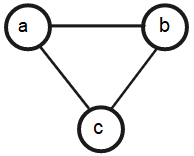
\includegraphics[width=2.3cm]{trianguloabc} && 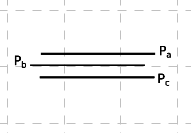
\includegraphics[width=3.5cm]{b0epgTransparenciaGrade2} & &
    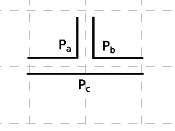
\includegraphics[width=3.5cm]{b1EpgTransparenteGrade2}
    \\
    \footnotesize
    (a) The  graph $C_3$ && \footnotesize(b) $B_0$-EPG representation of $C_3$ (edge-clique)&& \footnotesize(c) $B_1$-EPG representation of $C_3$ (claw-clique)\\
  \end{tabular}

 \caption{The  graph $ C_3 $  and  representations without bends and with 1 bend} \label{fig:trianguloepgRepresentacao}
\end{figure}

The \emph{bend number} of a graph $G$ is the smallest $k$ for which $G$ is a $B_k$-EPG graph. Analogously, the bend number of a class of graphs is the smallest $k$ for which all graphs in the class have a $B_k$-EPG representation. Interval graphs have bend number $0$, trees have bend number $1$, and outerplanar graphs have bend number $2$. The bend number for the class of planar graphs is still open, but it is either $3$ or $4$.

The class of EPG graphs has been studied in several papers, such as \cite{alcon2016, Asinowski2009, cohen2014, golumbic2009}, among others. The investigations regarding EPG graphs frequently approach characterizations concerning the number of bends of the graph representations. Regarding the complexity of recognizing $B_k$-EPG graphs, only the complexity of recognizing a few of these sub-classes of EPG graphs have been determined: $B_0$-EPG graphs can be recognized in polynomial time, since it corresponds to the class of interval graphs; in contrast, recognizing $B_1$-EPG and $B_2$-EPG graphs are NP-complete problems. 
Also, note that the paths in a $B_1$-EPG representation have one of the following shapes: $\llcorner$, $\lrcorner$, $\ulcorner$ and $\urcorner$. \cite{cameron2016edge} showed that for each $S\subset \{\llcorner, \lrcorner, \ulcorner, \urcorner\}$, it is NP-complete to determine if a given graph $G$ has a $B_1$-EPG representation using only paths with shape in $S$.

A  collection $C$ of sets satisfies the Helly property when every sub-collection of $C$ that is pairwise intersecting has at least one common element. 
The study of the Helly property is useful in diverse areas of science. We can enumerate applications in semantics, code theory, computational biology, database, image processing, graph theory, optimization, and linear programming.

The Helly property can also be applied to the $B_k$-EPG representation problem, where each path is considered a set of edges. A graph $G$ has a  Helly-$B_k$-EPG representation if there is a $B_k$-EPG representation of $G$ where each path has at most $k$ bends, and this representation satisfies the Helly property. Figure~\ref{fig:envelopeRepresentacoes}(a) presents two $B_1$-EPG representations of a graph with five vertices.  Figure~\ref{fig:envelopeRepresentacoes}(b)   illustrates 3 pairwise intersecting paths ($P_{v_1}, P_{v_2}, P_{v_5}$), containing a common edge, so it is a Helly-$B_1$-EPG representation. In Figure~\ref{fig:envelopeRepresentacoes}(c), although the three paths are pairwise intersecting, there is no common edge in all three paths, and therefore they do not satisfy the Helly property.

The Helly property related to EPG representations of graphs has been studied in~\cite{golumbic2009} and~\cite{golumbic2013}. 

Let $\cal {F}$ be a family of subsets of some universal set $U$, and $h\geq 2$ be an integer.  Say that $\cal{F}$ is $h$-{\it intersecting} when every group of $h$ sets of $\cal {F}$ intersect. The {\it core} of $\cal {F}$, denoted by $core(\cal F)$, is the intersection of all sets of $\cal {F}$. The family $\cal{F}$ is $h$-{\it Helly} when every $h$-intersecting subfamily $\cal{F'}$ of $\cal{F}$ satisfies $core(\cal{F'}) \neq \emptyset$. On the other hand, if for every subfamily $\cal{F'}$ of $\cal{F}$, there are $h$ subsets whose core equals the core of  $\cal {F'}$, then $\cal {F}$ is said to be {\it strong} $h$-{\it Helly}.
Note that the Helly property that we will consider in this paper is precisely the property of being 2-Helly. 

The  {\it Helly number} of the family $\cal{F}$ is the least integer $h$, such that $\cal{F}$ is $h$-Helly. Similarly, the {\it strong Helly number} of $\cal{F}$ is the least $h$, for which  $\cal{F}$ is strong $h$-Helly. It also follows that the strong Helly number of $\cal{F}$ is at least equal to its Helly number. In~\cite{golumbic2009} and~\cite{golumbic2013}, they have determined the strong Helly number of $B_1$-EPG graphs. 

\begin{figure}[h]
  \centering
  \begin{tabular}{ p{3.2cm} p{4.5cm} p{4.5cm} }
    \centering 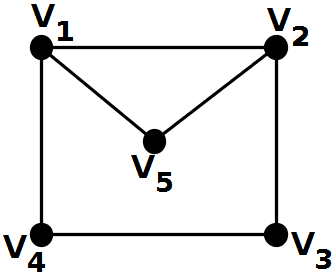
\includegraphics[width=3cm]{envelope} & 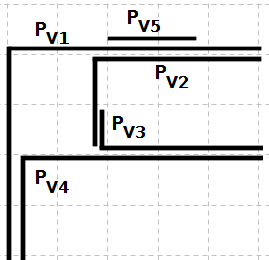
\includegraphics[width=4cm]{envelopeHellyGradeTransparente} & 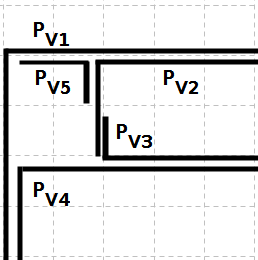
\includegraphics[width=4cm]{envelopeNaoHellyGrade}
    \\
    \footnotesize \centering (a) A  graph with 5 vertices & \footnotesize(b) $B_1$-EPG representation that satisfies the Helly property & \footnotesize (c) $B_1$-EPG representation that does  not satisfy the Helly property  \\

  \end{tabular}
\caption{A  graph with 5 vertices in (a) and some single bend representations: Helly in (b) and not Helly in (c)} \label{fig:envelopeRepresentacoes}
\end{figure}

%%%%%%%%%%%%%%%%%%%%%%%%%%%%%%%%%%%%%%%%%%%%%%%%%%%%%%%%%%%%%

% Next, we describe some terminology and notation.

% The term \emph{grid} is used to denote the Euclidean space of integer orthogonal coordinates. Each pair of integer coordinates corresponds to a \emph{point} (or vertex) of the grid. The \emph{size} of a grid is its number of points. The term \emph{edge of the grid} will be used to denote a pair of vertices that are at a distance one in the grid. Two edges $e_1$ and $e_2$ are \emph{consecutive edges} when they share exactly one point of the grid.
%  A (simple) path in the grid is as a sequence of distinct edges $e_1, e_2, \leq, e_m$,  where consecutive edges are adjacent, i.e., contain a common vertex, whereas non-consecutive edges are not adjacent.  In this context, two paths only intersect if they have at least a common edge. The first and last edges of a path are called \emph{extremity edges}.
  
% The \emph{direction of an edge} is vertical when the first coordinates of its vertices are equal, and is horizontal when the second coordinates are equal. A \emph {bend} in a path is a pair of consecutive edges $ e_1, e_2 $ of that path, such that the directions of $ e_1$ and $ e_2$ are different. When two edges $ e_1$ and $e_2 $ form a bend, they are called \emph { bend edges}. A \emph {segment} is a set of consecutive edges with no bends. %is a path with no bends.
% Two paths are said to be \emph{edge-intersecting}, or simply  \emph{intersecting} if they share at least one edge. Throughout the paper, any time we say that two paths intersect, we mean that they edge-intersect. If every path in a representation of a graph $G$ has at most $k$ bends, we say that this graph $G$ has a \emph{$B_k$-EPG} representation. When $k = 1$ we say that this is a \emph{single bend} representation.

% \medskip

% In this paper, we study the Helly-$B_k$-EPG graphs. First, we show that every graph admits an EPG representation that is Helly, and present a characterization of Helly-$B_1$-EPG representations. Besides, we relate Helly-$B_1$-EPG graphs with L-shaped graphs, a natural family of subclasses of $B_1$-EPG. Finally, we prove that recognizing Helly-$B_k$-EPG graphs is in NP, for every fixed $k$. Besides, we show that recognizing Helly-$B_1$-EPG graphs is NP-complete, and it remains NP-complete even when restricted to 2-apex and 3-degenerate graphs.

% The rest of the paper is organized as follows. In Section~\ref{sec:prelim}, we present some preliminary results, we show that every graph is a Helly-EPG graph, present a characterization of Helly-$B_1$-EPG representations, and relate Helly-$B_1$ EPG with L-shaped graphs. In Section~\ref{sec:NPpert}, we discuss the NP-membership of {\sc Helly-$B_k$ EPG Recognition}. In Section~\ref{sec:sectionDispositivoClausula}, we present the NP-completeness of recognizing Helly-$B_1$-EPG graphs.

Below we present the list of papers developed and published throughout my doctoral research, related to thesis. Some of these manuscripts and corresponding research was done while the author of this doctoral thesis was a doctoral research fellow at the National University of La Plata - UNLP, Math Department.

\begin{enumerate}
    
     \item BORNSTEIN, C. F.; GOLUMBIC, M.C.; SANTOS, T. D.; SOUZA, U. S.; SZWARCFITER, J. L.  The Complexity of Helly-B1-EPG graph Recognition. In: Discrete Mathematics \& Theoretical Computer Science (DMTCS), Source: oai:arXiv.org:1906.11185, June 4, 2020,  vol. 22 no. 1. 
     
     \item BORNSTEIN, C. F.; MORGENSTERN, G.; SANTOS, T. D.; SOUZA, U. S.; SZWARCFITER, J. L.  Helly and Strong Helly Numbers of $B_k$-EPG and $B_k$-VPG Graphs. Submitted to journal Discussiones Mathematicae Graph Theory (DMGT) on  May 16, 2020. 
 
     \item ALCON, L.; MAZZOLENI, M. P.;  SANTOS, T. D. Relationship Among $B_1$-EPG, VPT and EPT Graphs Classes. Accepted for publication in journal Discussiones Mathematicae Graph Theory (DMGT) on March 09, 2021.
\end{enumerate}

The following are  published/submitted papers in Conferences, Symposia and Congresses: 

\begin{enumerate}
    \item BORNSTEIN, C. F.; SANTOS, T. D.; SOUZA, U. S.; SZWARCFITER, J. L. A Complexidade do Reconhecimento de Grafos B1-EPG-Helly. In: 50º SBPO - Simpósio Brasileiro de Pesquisa Operacional, 2018, Rio de Janeiro. Cidades Inteligentes: Planejamento Urbano, Fontes Renováveis e Distribuição de Recursos, 2018.

     \item BORNSTEIN, C. F.; SANTOS, T. D.; SOUZA, U. S.; SZWARCFITER, J. L. Sobre a Dificuldade de Reconhecimento de Grafos B1-EPG-Helly. In: XXXVIII Congresso da Sociedade Brasileira de Computação, 2018, Natal - RN. Computação e Sustentabilidade, 2018. p. 113-116.

     
     \item BORNSTEIN, C. F.; SANTOS, T. D.; SOUZA, U. S.; SZWARCFITER, J. L. The complexity of B1-EPG-Helly graph recognition. In: VIII Latin American Workshop On Cliques in Graphs (LAWCG), ICM 2018 Satellite Event, 2018, Rio de Janeiro. Program and Abstracts, 2018. p. 69.
    
    \item ALCON, L.; MAZZOLENI, M. P.;  SANTOS, T. D. Identifying Subclasses of Helly-$B_1$-EPG Graphs.  52nd  Brazilian Operational Research Symposium (SBPO), 2020.
     
    \item ALCON, L.; MAZZOLENI, M. P.;  SANTOS, T. D. On Subclasses of Helly-$B_1$-EPG Graphs.   Reunión Anual de la Unión Matemática Argentina (virtUMA), 2020.
    
    \item ALCON, L.; MAZZOLENI, M. P.;  SANTOS, T. D. Paths on Hosts: $B_1$-EPG, EPT and VPT Graphs. Submitted to: 
    Latin American Workshop on Cliques in Graphs (LAWCG), 2020.
    
\end{enumerate}

The main results of this work are briefly presented as follows.

\section{The Helly property and EPG graphs}
The first group of studied problems involve two important widely addressed in the literature: the Helly property and EPG graphs. In this section we demonstrate that  every graph is an EPG graph and we present some subclasses of $B_1$-EPG graphs that are incomparable with Helly-$B_1$ EPG.  We present a characterization of Helly-$B_1$-EPG representations, and finally we demonstrate the $NP$-completness of the Helly-$B_k$ EPG recognition problem.

 \begin{lemma}\label{lem:todoGrafoEpgHelly}
 Every graph is a Helly-EPG graph.
 \end{lemma}
 
 \begin{corollary}\label{cor:maxCliques}
For every graph $G$ containing $\mu$ maximal cliques, it holds that $b_H(G)\leq \mu -1$. 
\end{corollary}

\begin{theorem}\label{theo:HellyLShaped}
$[\llcorner]\subsetneq [\llcorner, \urcorner]\subsetneq$~Helly-$B_1$ EPG, and Helly-$B_1$ EPG is incomparable with $[\llcorner, \ulcorner]$ and $[\llcorner, \ulcorner, \urcorner]$.
\end{theorem}

\begin{lemma}[\cite{golumbic2009}]\label{edge-claw-clique} 
Consider a $B_1$-EPG representation of a graph $G$. Every clique in $G$ corresponds to either an edge-clique or a claw-clique.
\end{lemma}

\begin{lemma}\label{caracterization}
A $B_1$-EPG representation of a graph $G$ is Helly if and only if each clique of $G$ is represented by an edge-clique, i.e., it does not contain any claw-clique.
\end{lemma}

The {\sc Helly-$B_k$ EPG recognition} problem can be formally described as follows.

\begin{table}[h!]
\centering
%\caption{My caption}
%\label{my-label}
\begin{tabular}{ll}
\hline \hline
\multicolumn{2}{c}{\sc Helly-$B_k$ EPG Recognition}                         \\ \hline \hline 
\emph{Input}: & A graph $G$ and an integer $k \leq |V(G)|^c$, for some fixed $c$.\\
~ & ~ \\
\emph{Goal:}  & \begin{tabular}[c]{@{}p{9.5cm}}
Determine if there is a set of $k$-bend paths \\ $\mathcal{P} = \{P_1, P_2, \ldots, P_n\} $ in a grid $ Q $ 
such that:\\ 
$\bullet$ \ \ \ $u,v\in V(G)$ are adjacent in $G$ if only if $P_u,P_v$\\ \hspace{0.6cm} share an edge in $Q$; and\\
$\bullet$ \ \ \ $\mathcal{P}$ satisfies the Helly property.
\end{tabular} \\ \hline
\end{tabular}
\end{table}

\begin{theorem}\label{teo:nppertinencia}
{\sc Helly-$B_k$ EPG recognition} is in NP.
\end{theorem}
\vspace{0.08cm}
\begin{theorem}
{\sc Helly-$B_1$ EPG recognition} is NP-complete.
\end{theorem}

\begin{corollary}\label{coro:2apexAnd3degenerate}
{\sc Helly-$B_1$ EPG recognition} is NP-complete on $2$-apex and $3$-degenerate graphs.
\end{corollary}

\section{Helly and Strong Helly Numbers of  $B_k$-EPG and $B_k$-VPG Graphs}
In this section, we solve the problem for determining the Helly and strong Helly numbers, for both $B_k$-EPG and $B_k$-VPG graphs, for each value $k$.

For EPG graphs,  the Helly number of  $B_0$-families is well known and is equal to 2, since $B_0$-EPG graphs coincide with interval graphs. It is also simple to conclude that the strong Helly number of $B_0$-EPG graphs are also equal to 2. For $k = 1$,  we prove that both the Helly number and the strong Helly number of the class of $B_1$-families are equal to 3. For the class of $B_2$-families, we prove that these two parameters are equal to 4. The Helly and strong Helly number for $B_3$-families equal 8, and finally, these parameters are unbounded for $k \geq 4$. 

As for VPG graphs, it is simple to verify that the Helly number of $B_0$-VPG graphs equals 2, and we prove that $B_1$-VPG have Helly number 4, $B_2$-VPG graphs have Helly number 6, $B_3$-VPG has Helly number 12, while the Helly number for $B_4$-VPG graphs is again unbounded. 

Finally, the strong Helly number equals the Helly number of $B_k$-EPG graphs, for each $k$. Similarly, for $B_k$-VPG graphs. 


As for existing results, 
Golumbic, Lipshteyn, and Stern \cite{golumbic2009}  have already shown that the strong Helly number for $B_1$-EPG graphs equal 3, and for $B_1$-VPG graphs is equal to 4. employing a different proof technique. See  \cite{golumbic2019edge}, Theorem 11.13, below:
\begin{theorem}\label{thm:golumbic2019edge}{\cite{golumbic2019edge}}
Let $P$ be a collection of single bend paths on a grid. If every two paths in $P$ share at least one grid-edge, then $P$ has strong Helly number 3. Otherwise, $P$ has strong Helly number 4.
\end{theorem}
No other results concerning the strong Helly number, or no results for the Helly number of $B_k$-EPG graphs seem to have been reported in the literature. As for other classes, Golumbic and Jamison have determined the strong Helly number of the intersection of edge paths of a tree \cite{golumbic1985}. Finally, Asinowski, Cohen, Golumbic, Limouzy, Lipshteyn, and Stern have reported that the strong Helly number of $B_0$-VPG graphs equals two.  


% GLM09  -> golumbic2009
% GJ85 -> golumbic1985
% A--11 -> asinowski2011string

% \begin{theorem}\label{thm:Helly-EPG}
% The Helly number of $B_k$-EPG graphs satisfy:
% \begin{enumerate}[nosep,label=\emph{(\roman*)}]
% \item  $H(B_1$-EPG) = 3 
% \item $H(B_2$-EPG)  = 4 
% \item $H(B_3$-EPG)  = 8 
% \item $H(B_k$-EPG) is unbounded, for 
% $k \geq 4$.
% \end{enumerate}

% \end{theorem}

% \begin{theorem}\label{thm:Bk-VPG}
% The Helly numbers for $B_k$-VPG graphs satisfy:
% \begin{enumerate}
% \item $H(B_1$-VPG) = 4
% \item $H(B_2$-VPG) = 6
% \item $H(B_3$-VPG) = 12
% \item $H(B_4$-VPG) is unbounded.
% \end{enumerate}
% \end{theorem}

Table \ref{tab:Helly-Strong-Helly} summarizes the results obtained.

\begin{table}[htb]
    \centering
    \begin{tabular}{c|c|c}
    \cline{1-3} $k$  & $B_k$-EPG & $B_k$-VPG \\
    \cline{1-3} 0 & 2 & 2 \\
    \cline{1-3} 1 & 3 & 4 \\
    \cline{1-3} 2 & 4 & 6 \\
    \cline{1-3} 3 & 8 & 12 \\
    \cline{1-3} $\geq 4$ & unbounded & unbounded \\
    \cline{1-3} 
    \end{tabular}
    \caption{Helly and Strong Helly Numbers for $B_k$-EPG and $B_k$-VPG Graphs}
    \label{tab:Helly-Strong-Helly}
\end{table}

\section{Relationship among  $B_1$-EPG, EPT and VPT graph classes}

In this section, we have considered three different path-intersection graph classes: $B_1$-EPG, VPT and EPT graphs. We showed that  $\{S_3, S_{3'},S_{3''},C_4\}$-free graphs and others non-trivial subclasses of  $B_1$-EPG graphs are Helly-$B_1$-EPG, namely by instance Bipartite, Block, Cactus and Line of Bipartite graphs. 
  
 We presented an infinite family of forbidden induced subgraphs for the class  $B_1$-EPG and in particular we proved  that Chordal $B_1$-EPG $\subset$ VPT $\cap$ EPT.  
 
 \begin{theorem}
\label{lem:chordalDiamondFree}
Let $G$ be a $B_1$-EPG graph. If $G$ is  $\{S_{3}, S_{3'}, S_{3''}, C_{4}\}$-free then $G$  is a Helly-$B_1$-EPG graph.
\end{theorem}

\begin{theorem} \label{lem:b1DiamondFree}
 If $G$ is a $B_1$-EPG and diamond-free graph then $G$ is a Helly-$B_1$-EPG graph.
 \end{theorem}
 
 \begin{cor}
If $G$ is a Bipartite $B_1$-EPG graph then $G$ is a Helly-$B_1$-EPG graph.
\end{cor}

\begin{cor}\label{lem:cdf}
 Block, Cactus and Line of Bipartite graphs are Helly-$B_1$-EPG.
\end{cor}

% \begin{cor}
%  graphs are  Helly-$B_1$-EPG.
% \end{cor}

% \begin{cor}\label{coro:lineOfBipartite}
%   graphs are Helly-$B_1$-EPG.
% \end{cor}
 
 \begin{theorem}\label{teo:chordalB1inVPT}
Chordal $B_1$-EPG $\subsetneq$ VPT. 
\end{theorem}

\begin{theorem}\label{teo:b1epgept}
Chordal $B_1$-EPG $\subsetneq$ EPT. 
\end{theorem}



% In this section, we have considered three different path-intersection graph classes: $B_1$-EPG, VPT and EPT graphs. We showed that  $\{S_3, S_{3'},S_{3''},C_4\}$-free graphs and others non-trivial subclasses of  $B_1$-EPG graphs are Helly-$B_1$-EPG, namely by instance Bipartite, Block, Cactus and Line of Bipartite graphs. 
  
%  We presented an infinite family of forbidden induced subgraphs for the class  $B_1$-EPG and in particular we proved  that Chordal $B_1$-EPG $\subset$ VPT $\cap$ EPT.  
 
 In~\cite{ries2009}, Asinowski and Ries described the   Split graphs that are $B_1$-EPG graphs in case the stable set  or the  central  size have size three. 
The graphs $F_2, F_{11}, F_{13}, F_{14}$ and $F_{15}$, given in~\cite{leveque2009characterizing} are Split, we have  used a different approach  to prove that they are not $B_1$-EPG graphs. So one question is pertinent: Can we characterize Split graphs in general based on the results of this section? 

\section{Concluding Remarks}
In this work, we present important contributions to issues involving intersection graphs, in particular EPG, VPG, EPT and VPT graph classes. In addition, our research ventures into several areas of science when it solves classic problems such as the definition of bounds for parameters in Mathematics and Graph Theory, but it also presents results as proof of hardness in the  $NP$-Completness Theory.

In addition to the publications cited throughout the text, we also have a paper to be published in the jornal \textit{"Matemática Contemporânea"} whose the title \textit{"On Helly-B1-EPG graphs"}. There is also a continuation of research in progress, on intersection graphs with a new type of grid, now triangular.

\bibliographystyle{sbc}
\bibliography{sbc-template}

\end{document}
